%& C:\Users\Peter\AppData\Roaming\TikzEdt\TikzEdt\023~1.0\TEMP_H~1
\begin{document}
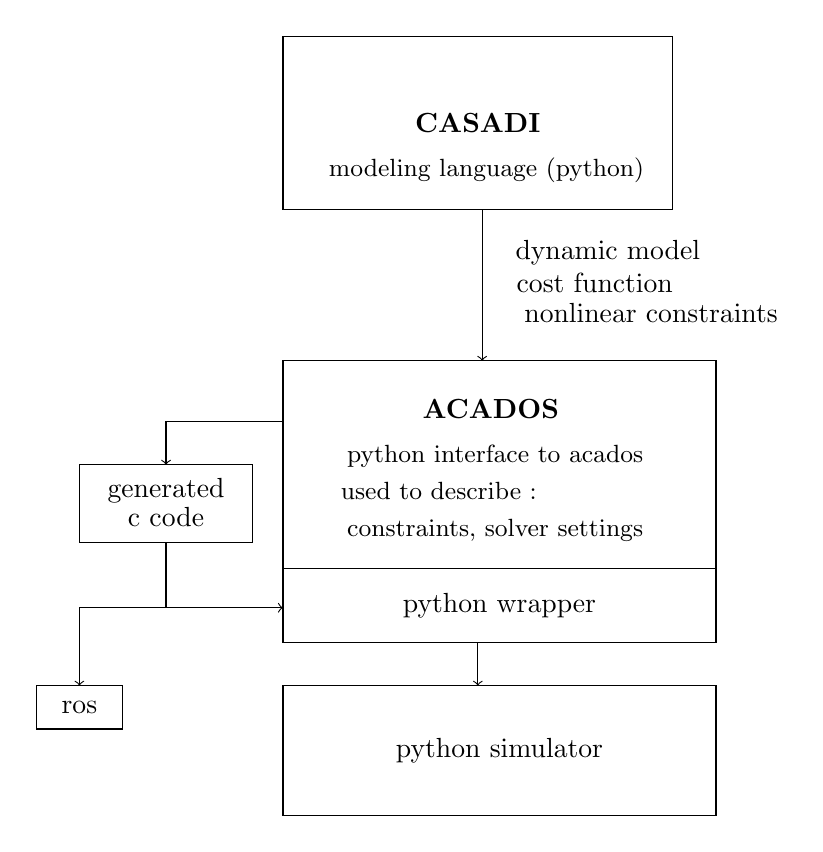
\begin{tikzpicture}[scale=1.1]
\draw  (-2.5,4.5) rectangle (2,2.5) node [pos=.5]{\bf CASADI};
\node at (-0.15,2.95) {\small modeling language  (python)};
\draw[->] (-0.2,2.5) -- (-0.2,0.75);
\node at (1.25,2) {dynamic model};
 
\draw  (-2.5,0.75) rectangle (2.5,-2.5) {};

\node at (-0.05,-0.35) {\small python interface to acados};
\node[minimum width=1.5cm] at (-0.7,-0.75) {\small used to describe : };
\node at (-0.05,-1.2) {\small constraints, solver settings};
\node at (1.1,1.65) {cost function};
\node at (1.75,1.3) {nonlinear constraints};
\node at (-0.1,0.2) {\bf ACADOS};

\draw  (-4.85,-0.45) rectangle (-2.85,-1.35);
\node at (-3.85,-0.75) {generated };
\node at (-3.85,-1.05) {c code};
\draw[->] (-2.5,0.05) -- (-3.85,0.05) -- (-3.85,-0.45);
\draw[->] (-3.85,-1.35) -- (-3.85,-2.1) -- (-2.5,-2.1);
\draw[->] (-3.85,-2.1) -- (-4.85,-2.1) -- (-4.85,-3);
\draw  (-5.35,-3) rectangle (-4.35,-3.5)node[pos=.5]{ros};
\draw  (-2.5,-1.65) rectangle (2.5,-2.5)node[pos=.5]{python wrapper};
\draw  (-2.5,-3) rectangle (2.5,-4.5)node[pos = .5]{python simulator};
\draw[->] (-0.25,-2.5) -- (-0.25,-3);

\usetikzlibrary{calc}
\pgftransformreset
\node[inner sep=0pt,outer sep=0pt,minimum size=0pt,line width=0pt,text width=0pt,text height=0pt] at (current bounding box) {};
%add border to avoid cropping by pdflibnet
\foreach \border in {0.1}
  \useasboundingbox (current bounding box.south west)+(-\border,-\border) rectangle (current bounding box.north east)+(\border,\border);
\newwrite\metadatafile
\immediate\openout\metadatafile=\jobname_BB.txt
\path
  let
    \p1=(current bounding box.south west),
    \p2=(current bounding box.north east)
  in
  node[inner sep=0pt,outer sep=0pt,minimum size=0pt,line width=0pt,text width=0pt,text height=0pt,draw=white] at (current bounding box) {
\immediate\write\metadatafile{\p1,\p2}
};
\immediate\closeout\metadatafile
\end{tikzpicture}

\end{document}
